\documentclass[12pt]{article}

\usepackage{amsmath, mathtools}
\usepackage{amsfonts}
\usepackage{amssymb}
\usepackage{graphicx}
\usepackage{colortbl}
\usepackage{xr}
\usepackage{hyperref}
\usepackage{longtable}
\usepackage{xfrac}
\usepackage{tabularx}
\usepackage{float}
\usepackage{siunitx}
\usepackage{booktabs}
\usepackage{caption}
\usepackage{pdflscape}
\usepackage{afterpage}

\usepackage[round]{natbib}

%\usepackage{refcheck}

\hypersetup{
    bookmarks=true,         % show bookmarks bar?
      colorlinks=true,       % false: boxed links; true: colored links
    linkcolor=red,          % color of internal links (change box color with linkbordercolor)
    citecolor=green,        % color of links to bibliography
    filecolor=magenta,      % color of file links
    urlcolor=cyan           % color of external links
}

%% Comments

\usepackage{color}

\newif\ifcomments\commentstrue

\ifcomments
\newcommand{\authornote}[3]{\textcolor{#1}{[#3 ---#2]}}
\newcommand{\todo}[1]{\textcolor{red}{[TODO: #1]}}
\else
\newcommand{\authornote}[3]{}
\newcommand{\todo}[1]{}
\fi

\newcommand{\wss}[1]{\authornote{blue}{SS}{#1}}
\newcommand{\an}[1]{\authornote{magenta}{Author}{#1}}


% For easy change of table widths
\newcommand{\colZwidth}{1.0\textwidth}
\newcommand{\colAwidth}{0.13\textwidth}
\newcommand{\colBwidth}{0.82\textwidth}
\newcommand{\colCwidth}{0.1\textwidth}
\newcommand{\colDwidth}{0.05\textwidth}
\newcommand{\colEwidth}{0.8\textwidth}
\newcommand{\colFwidth}{0.17\textwidth}
\newcommand{\colGwidth}{0.5\textwidth}
\newcommand{\colHwidth}{0.28\textwidth}

% Used so that cross-references have a meaningful prefix
\newcounter{defnum} %Definition Number
\newcommand{\dthedefnum}{GD\thedefnum}
\newcommand{\dref}[1]{GD\ref{#1}}
\newcounter{datadefnum} %Datadefinition Number
\newcommand{\ddthedatadefnum}{DD\thedatadefnum}
\newcommand{\ddref}[1]{DD\ref{#1}}
\newcounter{theorynum} %Theory Number
\newcommand{\tthetheorynum}{T\thetheorynum}
\newcommand{\tref}[1]{T\ref{#1}}
\newcounter{tablenum} %Table Number
\newcommand{\tbthetablenum}{T\thetablenum}
\newcommand{\tbref}[1]{TB\ref{#1}}
\newcounter{assumpnum} %Assumption Number
\newcommand{\atheassumpnum}{P\theassumpnum}
\newcommand{\aref}[1]{A\ref{#1}}
\newcounter{goalnum} %Goal Number
\newcommand{\gthegoalnum}{P\thegoalnum}
\newcommand{\gsref}[1]{GS\ref{#1}}
\newcounter{instnum} %Instance Number
\newcommand{\itheinstnum}{IM\theinstnum}
\newcommand{\iref}[1]{IM\ref{#1}}
\newcounter{reqnum} %Requirement Number
\newcommand{\rthereqnum}{P\thereqnum}
\newcommand{\rref}[1]{R\ref{#1}}
\newcounter{lcnum} %Likely change number
\newcommand{\lthelcnum}{LC\thelcnum}
\newcommand{\lcref}[1]{LC\ref{#1}}
\newcounter{calcnum} %Calculation Number
\newcommand{\cthecalcnum}{C\thecalcnum}
\newcommand{\cref}[1]{C\ref{#1}}
\newcounter{outputnum} %Output Number
\newcommand{\otheoutputnum}{O\theoutputnum}
\newcommand{\oref}[1]{O\ref{#1}}
\newcounter{bibnum} %Output Number
\newcommand{\bthebibnum}{\thebibnum}
\newcommand{\bref}[1]{\ref{#1}}
\newcounter{nfrnum} %NFR Number
\newcommand{\nfrthenfrnum}{\thenfrnum}
\newcommand{\nfrrref}[1]{NFR\ref{#1}}


\newcommand{\progname}{Linear Algebraic Equation Solver} % PUT YOUR PROGRAM NAME HERE

\usepackage{fullpage}

\begin{document}

\title{Commonality Analysis for a Library of Linear Algebraic Equation Solver } 
\author{Devi Prasad Reddy Guttapati}
\date{October 4, 2017}
	
\maketitle
\pagebreak
\pagenumbering{roman}
\tableofcontents

\begin{table}[bp]
\caption{\bf Revision History}
\begin{tabularx}{\textwidth}{p{3cm}p{2cm}X}
\toprule {\bf Date} & {\bf Version} & {\bf Notes}\\
\midrule
October 4, 2017 & 1.0 & Initial Draft\\

\bottomrule
\end{tabularx}
\end{table}

\section{Reference Material}



\subsection{Table of Units}

This section does not apply to this program family.

\subsection{Table of Symbols}

The table that follows summarizes the symbols used in this document along with
their units.  The choice of symbols was made to be consistent with the heat
transfer literature and with existing documentation for solar water heating
systems.  The symbols are listed in alphabetical order.

\renewcommand{\arraystretch}{1.2}
%\noindent \begin{tabularx}{1.0\textwidth}{l l X}
\noindent \begin{longtable*}{l l p{12cm}} \toprule
\textbf{symbol} & \textbf{unit} & \textbf{description}\\
\midrule


$A$ & \text{-} & known \textit{m $\times$ n} matrix \wss{Remove texit, just use
  equation environment.}\\
$x$ & \text{-} & \textit{n}-vector\\
$b$ & \text{-} & \textit{m}-vector\\
M$_{1}$ & \text{-} & elementary elimination matrix\\
$L$ & \text{-} & lower triangular matrix\\
$U$ & \text{-} & upper triangular matrix\\ 
A$^{-1}$ & \text{-} & inverse of matrix \\
$I$ & \text{-} & identity matrix\\
{${|A|}$} & \text{-} & determinant of matrix\\ 

\bottomrule
\end{longtable*}


\subsection{Abbreviations and Acronyms}

\renewcommand{\arraystretch}{1.2}
\begin{tabular}{l l} 
  \toprule		
  \textbf{symbol} & \textbf{description}\\
  \midrule 
  A & Assumption\\
  DD & Data Definition\\
  GD & General Definition\\
  GS & Goal Statement\\
  IM & Instance Model\\
  LC & Likely Change\\
  PS & Physical System Description\\
  R & Requirement\\
  SRS & Software Requirements Specification\\

  T & Theoretical Model\\
  O & Output\\
  \bottomrule
\end{tabular}\\



\newpage
\pagenumbering{arabic}

\section{Introduction}

Many of the relationships in nature are linear, that means their effects are
proportional to their causes. For example in Mechanics if we take Newtons second
law of motion, \textbf{F = ma} says that force is proportional to acceleration
and mass is the proportionality constant. For example in Electricity if we take
Ohm's Law, \textbf{V = iR} voltage across the conductor is proportional to the
current flowing though it and resistance is the proportionality constant. These
examples shows us the importance of linear equations and solving them. In matrix
notation the general form of linear equation is

 \centerline{\textbf{Ax = b}}

where \textbf{A} is known \textit{m $\times$ n} matrix, \textbf{b} is an
\textit{m}-vector and \textbf{x} is an \textit{n}-vector. If \textbf{x} is
known, then such a linear relationship enables us to predict effect \textbf{b}
from cause \textbf{x} by matrix-vector multiplication \textbf{b} =
\textbf{A}\textbf{x}.

The most important problem in technical computing is the solution of system
linear equations.



\subsection{Purpose of Document}

The purpose of the document is to describe the methods and process for solving
the family of linear algebraic equations. A study on the method for solution of
system of linear equations and the problems effecting the effectiveness and
efficiency will be detected and correct recommendations will be made. The
significance of this document is to make a solution technique for solving family
of linear equations easier and to reduce stress on the human brain associated
with lots of reasoning when solving linear equation.

This document also describes General System Description, Commonalities,
Variabilities.

\subsection{Scope of the Family} 

The scope of the family is limited to the library of linear algebraic equation
solvers. If the user gives proper input the linear algebraic equation solver
aims to solve the equations and give the correct output.

\subsection{Characteristics of Intended Reader} 

The intended readers who read this document must have basic knowledge about
linear algebraic equations and the different methods of solving linear algebraic
equations which are typically covered in first and second year Linear Algebra
courses . \wss{Watch the spacing in your sentences with punctuation.}

\subsection{Organization of Document}

The template for Commonality Analysis for scientific computing software is
proposed by~\cite{smith2006systematic}. The document is organized perfectly step
by step right from the introduction to the appendix by explaining the important
concepts like General System Description, Commonalities, Variabilities.

\section{General System Description}

This section identifies the interfaces between the system and its environment,
describes the user characteristics and lists the system constraints.

\subsection{System Context}

\begin{figure}[h]
\centering
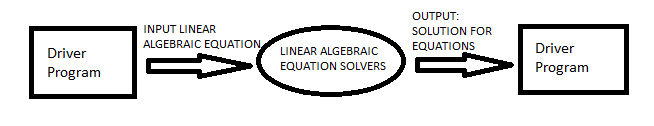
\includegraphics[scale= .7]{diagram1}
\caption{System Context}
\end{figure}



The figure shows the system context. The user gives the input in the form of
linear equations to the solver and the solver aims to give the solution to the
equations as the output.

\wss{The user likely makes more sense as program rather than a person.}

\begin{itemize}
\item User Responsibilities:
\begin{itemize}
\item The main responsibility of the user is to give the appropriate input.
\item User must make sure that the input given is error free.
\item User must enter the values in matrix form. \wss{Does the user really need
    to put the data in the correct format?  If it isn't in the correct software,
    the software should be able to detect this.}
\end{itemize}
\item \progname{} Responsibilities:
\begin{itemize}
\item The main responsibility of the linear algebraic equation solver is to
  identify the input which is improper or invalid. \wss{This point shows that
    your software does check the format, so you don't need the last point in the
    user responsibility list.}
\item Detect data type mismatch, such as a string of characters instead of a
  floating point number.
\item the ultimate responsibility of the linear algebraic equation solver is to
solve the equations and to produce the output.
\end{itemize}
\end{itemize}

\subsection{User Characteristics} \label{SecUserCharacteristics}

The end user of \progname{} should have an understanding of undergraduate Level
of linear algebra.  \wss{What level course?  Mathematics is quite standardized,
  so saying Linear Algebra 1, would be helpful.}

\subsection{System Constraints}

There are no system constraints applicable.

\section{Commonalities}

This section first presents the problem description, which gives a high-level
view of the problem to be solved. This is followed by the Terminology and
Definitions, Data Definitions, Goal Statements and Theoretical Models.

\subsection{Problem Description} \label{Sec_pd}

\progname{} is a software library which is developed to solve linear algebraic equations using numerical methods for linear algebraic equation . This solver is used to solve the linear algebraic equations with different number of variables. As many relationships in nature are linear, it will be very handy for
students to solve linear algebraic equations.

\subsection{Terminology and  Definitions}

This subsection provides a list of terms that are used in the subsequent
sections and their meaning, with the purpose of reducing ambiguity and making it
easier to correctly understand the requirements:




\begin{itemize}

\item \textbf{A} is a known \textit{m $\times$ n} matrix 

\item \textbf{b} is an \textit{m}-vector 

\item \textbf{x} is an \textit{n}-vector

\item \textbf{A$^{-1}$} is the inverse of the matrix \textbf{A}

\item rank(\textbf{A}) = \textit{n} the rank of a matrix is the maximum number
of linearly independent rows or columns it contains. \wss{the rank of a matrix
  is not always $n$.}

\item det(\textbf{A}) is determinant of matrix \textbf{A}


\end{itemize}

\wss{The terminology you have listed is mostly a repetition of symbols you are
  using elsewhere.  Terminology is more for definitions of terms.  You could
  define terms like singular, condition number etc.  Your definition of rank
  seems like an appropriate item to list here.  The information above is a
  better fit for the list of symbols.}

\pagebreak

\subsection{Data Definitions} \label{sec_datadef}

~\newline

\noindent
\begin{minipage}{\textwidth}
\renewcommand*{\arraystretch}{1.5}
\begin{tabular}{| p{\colAwidth} | p{\colBwidth}|}
\hline
\rowcolor[gray]{0.9}
Number& DD\refstepcounter{datadefnum}\thedatadefnum \label{D_matrix}\\
\hline
Label& \bf Matrix Representation of the Linear Algebraic Equation\\
\hline
Symbol & \textbf{Ax = b}\\
\hline

  Equation&\[
\left\{ 
\begin{array}{c}
ax_1+bx_2=b_1 \\ 
cx_1+dx_2=b_2 \\ 

\end{array}
\right. 
\]\\
  \hline
  Description 
        &\textbf{A} is a known \textit{m x n} matrix that is 
$\begin{bmatrix}
  a & b\\
  c & d
\end{bmatrix}$.\\
        & \textbf{b} is an \textit{m}-vector that is
$\begin{bmatrix}
  b_1\\
  b_2
\end{bmatrix}$.\\
        &\textbf{x} is an \textit{n}-vector that is 
$\begin{bmatrix}
  x_1\\
  x_2
\end{bmatrix}$. \wss{Your definitions are just for a two by two matrix.  You
  should explain what it means to have an $m \times n$ matrix.}\\
  \hline
  Source&
       Scientific Computing, An Introductory Survey, Second Edition by MICHEL
          \wss{spell check}
          T. HEATH, Chapter 2. \wss{Use BibTeX for this and put the reference in
          your list of references}
  \\
  \hline
  Ref.\ By & [\iref{gaussian}], [\iref{gauss}], [\tref{T_uniqsoln}],
             [\tref{T_LAE}], [\aref{A_explicit}], [\aref{A_matrixform}]
             \wss{I've had a look at some of these reference by items and they
             don't actually have references.  You have to actually use the
             references to put this in.}\\
  \hline
\end{tabular}
\end{minipage}\\


~\newline

\noindent
\begin{minipage}{\textwidth}
\renewcommand*{\arraystretch}{1.5}
\begin{tabular}{| p{\colAwidth} | p{\colBwidth}|}
\hline
\rowcolor[gray]{0.9}
Number& DD\refstepcounter{datadefnum}\thedatadefnum \label{D_inverse}\\
\hline
Label& \bf Inverse of a Matrix\\
\hline
Symbol & \textbf{A$^{-1}$}\\
\hline

  Equation&
\textbf{A}\textbf{A$^{-1}$} = \textbf{A$^{-1}$}\textbf{A} = \textbf{I}\\
  \hline
  Description 
        &\textbf{A} is a known \textit{m x n} matrix.\\


        & \textbf{A$^{-1}$} is the inverse of matrix \textbf{A} .\\
        &\textbf{I} is an Identity matrix . \wss{You should define the identity
          matrix somewhere.  It would be a good data definition.}\\
  \hline
  Source&
       Scientific Computing, An Introductory Survey, Second Edition by MICHEL T. HEATH, Chapter 2.
  \\
  \hline
  Ref.\ By & [\iref{gaussian}], [\iref{gauss}],  [\ddref{D_determinant}],  [\tref{T_uniqsoln}], [\aref{A_unique}] \\
  \hline
\end{tabular}
\end{minipage}\\

~\newline

\noindent
\begin{minipage}{\textwidth}
\renewcommand*{\arraystretch}{1.5}
\begin{tabular}{| p{\colAwidth} | p{\colBwidth}|}
\hline
\rowcolor[gray]{0.9}
Number& DD\refstepcounter{datadefnum}\thedatadefnum \label{D_determinant}\\
\hline
Label& \bf Determinant of a Matrix\\
\hline
Symbol & \textbf{${|A|}$}\\
\hline

  Equation&
 \textbf{$${|A|} = \sum_{i=1}^{k} a_{ij} C_{ij}$$}\\
  \hline
  Description 
        &\textbf{${|A|}$} is the determinant of matrix \textbf{A}.\\


        & \textbf{ C$_{ij}$} is the cofactor of {a$_{ij}$} defined by {C$_{ij}$} = {(-1)$^{i+j}$}{M$_{ij}$} .\\

        & {M$_{ij}$} is the minor of matrix A formed by eliminating row i and column j from A.\\
        
  \hline
  Source&
       \url{http://mathworld.wolfram.com/Determinant.html}\\
       

  \hline
  Ref.\ By & [\iref{gaussian}], [\iref{gauss}],  [\ddref{D_inverse}],  [\tref{T_uniqsoln}],  [\aref{A_unique}] \\
  \hline
\end{tabular}
\end{minipage}\\


~\newline

\noindent
\begin{minipage}{\textwidth}
\renewcommand*{\arraystretch}{1.5}
\begin{tabular}{| p{\colAwidth} | p{\colBwidth}|}
\hline
\rowcolor[gray]{0.9}
Number& DD\refstepcounter{datadefnum}\thedatadefnum \label{D_rank}\\
\hline
Label& \bf Rank of a Matrix\\
\hline
Symbol & \textbf{rank(A)}\\
\hline

  Equation&
 \textbf{rank(A) $\leq min(m, n)$}\\
  \hline
  Description 
        & rank(A) is the rank of matrix A.\\


        & We assume that A is an m $\times$ n matrix and we define the linear map f by f(x) = Ax  .\\

        & The rank of an m $\times$ n matrix is a nonnegative integer and cannot
          be greater than either m or n . \wss{You haven't really defined rank.}\\
        
  \hline
  Source&
       \url{https://www.cliffsnotes.com/study-guides/algebra/linear-algebra/real-euclidean-vector-spaces/the-rank-of-a-matrix}\\
       

  \hline
  Ref.\ By & [\iref{gaussian}], [\iref{gauss}],  [\tref{T_uniqsoln}],  [\aref{A_unique}]\\
  \hline
\end{tabular}
\end{minipage}\\



% \begin{figure}[h!]
% \begin{center}
% %\rotatebox{-90}
% {
%  \includegraphics[width=0.5\textwidth]{<FigureName>}
% }
% \caption{\label{<Label>} <Caption>}
% \end{center}
% \end{figure}

\subsection{Goal Statements}



\begin{itemize}

\item[GS\refstepcounter{goalnum}\thegoalnum \label{G_solveforx}:] {
Given the general linear algebraic equation problem which is represented by
\textbf{Ax = b}. The initial values are A and B. The input which are the coefficients, are entered in a matrix form. If the vector b of effects is known then it would likely able to determine the corresponding vector x of cause.}

%\item[GS\refstepcounter{goalnum}\thegoalnum \label{G_InputOutput}:]{
%The user must provide the required input there by calling the linear algebraic equation solver, and the solver must display the output.}
\end{itemize}




\subsection{Theoretical Models}\label{sec_theoretical}

This section focuses on the general equations and laws that \progname{} is based
on.  

~\newline

\noindent
\begin{minipage}{\textwidth}
\renewcommand*{\arraystretch}{1.5}
\begin{tabular}{| p{\colAwidth} | p{\colBwidth}|}
  \hline
  \rowcolor[gray]{0.9}
  Number& T\refstepcounter{theorynum}\thetheorynum \label{T_LAE}\\
  \hline
  Label&\bf General Linear Algebraic Equation\\
  \hline
  Equation&   \textbf{Ax = b}\\
  \hline
  Description & 
A linear transformation between two finite dimensional vector spaces is
represented by a matrix. In matrix-vector notation, a system of linear algebraic
equations has the form \textbf{Ax = b} where \textbf{A} is known \textit{m $\times$ n}
matrix, \textbf{b} is an \textit{m}-vector and \textbf{x} is an
\textit{n}-vector. If \textbf{x} is known, then such a linear relationship
enables us to predict effect \textbf{b} from cause \textbf{x} by matrix-vector
multiplication \textbf{b} = \textbf{A}\textbf{x}. The linear system will also
enable us to "reverse engineering", \wss{Use ``quote'' to get correct quotation
                marks} if we know the vector \textbf{b} of effects,
we can be able to determine the corresponding vector \textbf{x} of cause. \\
  \hline
  Source &
           \url{http://www.sciencedirect.com/science/article/pii/0377042794903026}\\
  % The above web link should be replaced with a proper citation to a publication
  \hline
  Ref.\ By &  [\iref{gaussian}], [\iref{gauss}], [\aref{A_explicit}], [\aref{A_matrixform}], [\cref{C_inputs}] \\
  \hline
\end{tabular}
\end{minipage}\\

\wss{You should introduce the assumption that $A$ is a square matrix here.
  There is no reason to continue with the more general $m \times n$ case.  (You
  should also add an explicit assumption that $A$ is square.  This is also
  something you should say in the scope section.)}

~\newline

\noindent
\begin{minipage}{\textwidth}
\renewcommand*{\arraystretch}{1.5}
\begin{tabular}{| p{\colAwidth} | p{\colBwidth}|}
  \hline
  \rowcolor[gray]{0.9}
  Number& T\refstepcounter{theorynum}\thetheorynum \label{T_uniqsoln}\\
  \hline
  Label&\bf Existence and Uniqueness\\
  \hline
  Equation&   \textbf{Ax = b}

An \textit{n $\times$ n} matrix \textbf{A} is said to be nonsingular if it satisfies any of the following equivalent conditions:


1. \textbf{A} has an inverse (there is a matrix, denoted by \textbf{A$^{-1}$},
such that \textbf{A}\textbf{A$^{-1}$} = \textbf{A$^{-1}$}\textbf{A} =
\textbf{I}, the identity matrix).


 2. Determinant of (\textbf{A}) is not equals to 0   

 3. rank(\textbf{A}) = \textit{n} (the rank of a matrix is the maximum number of
            linearly independent  rows or columns it contains).   \wss{If you
            have a list use the itemize or enumerate environments in LaTeX.}\\

  \hline
Description & The existence of a solution to a system of linear equations
\textbf{Ax = b} depend on whether the matrix \textbf{A} is singular or
nonsingular. If the matrix \textbf{A} is nonsingular, then its inverse
\textbf{A$^{-1}$} exists, and the system \textbf{Ax = b} always has a unique
solution \textbf{x} = \textbf{A$^{-1}$}\textbf{b} regardless of the value for b.
If the matrix \textbf{A} is singular, then the number of solutions is determined
by the right hand side vector \textbf{b}. \\
  \hline
  Source &
           \url{http://www.sciencedirect.com/science/article/pii/0377042794903026}\\
  % The above web link should be replaced with a proper citation to a publication
  \hline
Ref.\ By & [\iref{gaussian}], [\iref{gauss}], [\ddref{D_inverse}],
[\ddref{D_determinant}], [\ddref{D_rank}], [\aref{A_unique}], [\cref{C_inputs}]
\\
  \hline
\end{tabular}
\end{minipage}\\

~\newline

\wss{This shouldn't be a separate theoretical model.  It is part of the first
  model.  The potential solutions for a linear system of equations are a unique
  solution, an infinite number of solutions or no solution.  You should then
  reference definitions that define what rank, singular etc. mean.}

\section{Variabilities}

The instance models that govern \progname{} are presented in
Subsection 4.2.5.  The information to understand the meaning of the
instance models and their derivation is also presented, so that the instance
models can be verified.




\subsection{Instance Models} \label{sec_instance}    

This section transforms the problem defined in Section~\ref{Sec_pd} into 
one which is expressed in mathematical terms. 

~\newline

%Instance Model 1

\noindent
\begin{minipage}{\textwidth}
\renewcommand*{\arraystretch}{1.5}
\begin{tabular}{| p{\colAwidth} | p{\colBwidth}|}
  \hline
  \rowcolor[gray]{0.9}
  Number& IM\refstepcounter{instnum}\theinstnum \label{gaussian}\\
  \hline
  Label& \bf Gaussian Elimination Method for solving Linear Algebraic Equations\\
  \hline
  Input& \textbf{A}, \textbf{b}   \\
  
  \hline
  Output& \textbf{M$_1$}, \textbf{L}, \textbf{U}, \textbf{x} \wss{The output
          should only be $x$ and an element from enumerated type that indicates
          whether the matrix is singular or not.}   \\
  \hline
  Description&A is a known \textit{m $\times$ n} matrix.\\
  &x is an \textit{n}-vector.\\
  &b is an \textit{m}-vector.\\
  &M$_{1}$ is an elementary elimination matrix.\\
  &L is lower triangular matrix.\\
  & U is upper triangular matrix.
  \\
  \hline
  Sources& \url{http://www.sciencedirect.com/science/article/pii/0377042794903026}\\
  \hline
  Ref.\ By & [\aref{A_programcall}], [\aref{A_explicit}], [\aref{A_matrixform}], [\aref{A_unique}], [\aref{A_complex}], [\aref{A_entryofA}], [\aref{A_entryofb}]\\
  \hline
\end{tabular}
\end{minipage}\\

\wss{You are really inconsistent with the notation.  At some points you use bold
  face for matrices and vectors, other times you do not.  You also are not
  consistent in putting your variables and equations in the LaTeX equation
  environment.}

\subsubsection*{Derivation of Gaussian Elimination Method}{

It is fairly simple matter to reduce a general linear system \textbf{Ax = b} to
upper triangular form. We first choose an elementary elimination matrix
\textbf{M$_1$} with the first diagonal entry \textbf{a$_{11}$} as pivot, so that
the first column of \textbf{A} becomes zero below the first row when
premultiplied by \textbf{M$_1$}. All the remaining columns of \textbf{A}, as
well as right-hand-side vector \textbf{b}, must also be multiplied by
\textbf{M$_1$}, so the new system becomes \textbf{M$_1$}\textbf{Ax} =
\textbf{M$_1$}\textbf{b}.

Next we use the second diagonal entry as pivot to determine a second elementary
elimination matrix \textbf{M$_2$} that annihilates all of the entries of the
second column of the new matrix, \textbf{M$_1$}\textbf{A}, below the second row.
Again, \textbf{M$_2$} must be applied to the entire matrix and right-hand-side
vector, so that we obtain the further modified linear system
\textbf{M$_2$}\textbf{M$_1$}\textbf{Ax} =
\textbf{M$_2$}\textbf{M$_1$}\textbf{b}. Note that the first column of the matrix
\textbf{M$_1$}\textbf{A} is not effected by \textbf{M$_2$} because all of its
entries are zero in the relevant rows. If we define the matrix \textbf{M} =
\textbf{M$_{n-1}$}...\textbf{M$_{1}$}, then the transformed the linear system is

\vspace{.5cm}

\textbf{M}\textbf{A}\textbf{x} = \textbf{M$_{n-1}$}...
\textbf{M$_{1}$}\textbf{A}\textbf{x} = \textbf{M$_{n-1}$}...
\textbf{M$_{1}$}\textbf{b} = \textbf{M}\textbf{b}

\vspace{.5cm}

is upper triangular and can be solved by back-substitution to obtain the
solution to the original linear system \textbf{Ax = b}.

The process we have just described is known as Gaussian elimination. It is also
known as LU factorization or LU decomposition because it decomposes the matrix
\textbf{A} into product of a unit lower triangular matrix, \textbf{L}, and the
upper triangular matrix, \textbf{U}. To see this, recall that the product
\textbf{L$_k$}\textbf{L$_j$} is unit lower triangular if k<j, so taht \wss{spell check!}

\vspace{.5cm}

\textbf{L} = \textbf{M$^{-1}$} =
\textbf{(\textbf{M$_{n-1}$}...\textbf{M$_{1}$})$^{-1}$} =
\textbf{{M$_{1}$}$^{-1}$}...\textbf{{M$_{n-1}$}$^{-1}$} =
\textbf{L$_{1}$}...\textbf{L$_{n-1}$}

\vspace{.5cm}

is unit lower triangular. We have already seen that, by design, the matrix
\textbf{U} = \textbf{MA} is upper triangular. Therefore, we have expressed
\textbf{A} as a product

\vspace{.5cm}

\textbf{A} = \textbf{LU}

\vspace{.5cm}

where \textbf{L} is unit lower triangular and \textbf{U} is upper triangular.
Given such a factorization, the linear system \textbf{Ax = b} can be written as
\textbf{LUx} = \textbf{b} and hence can be solved by first solving the lower
triangular system \textbf{Ly} = \textbf{b} by forward-substitution, then the
upper triangular matrix \textbf{Ux} = \textbf{y} by back-substitution.

In solving a linear system \textbf{Ax = b}, the necessary transformation of the
right-hand-side vector \textbf{b} could be included as a part of LU
factorization process, or it could be done as a separate step to solve the lower
triangular system \textbf{Ly} = \textbf{b} after \textbf{L} has been obtained.
In either case, back-substitution for upper triangular matrix is then used to
solve the upper triangular system \textbf{Ux} = \textbf{y} to obtain the
solution \textbf{x}.

\wss{The above text is plagiarized.  You cannot take someone else's words and
  present them as your own without citation.  The above is almost a direct quote
  from Heath, but you don't cite that resource here.  Please be very careful to
  not do this.  For the current project, it would have been fine to not produce
  all of these details.  You could give a high level overview of the algorithm
  and simply refer the reader to the Heath textbook for the details.}

~\newline

%Instance Model 2

\noindent
\begin{minipage}{\textwidth}
\renewcommand*{\arraystretch}{1.5}
\begin{tabular}{| p{\colAwidth} | p{\colBwidth}|}
  \hline
  \rowcolor[gray]{0.9}
  Number& IM\refstepcounter{instnum}\theinstnum \label{gauss}\\
  \hline
  Label& \bf Gauss-Jordan Elimination Method for solving Linear Algebraic Equations\\
  \hline
  Input&  \textbf{A}, \textbf{b}   \\
  
  \hline
  Output& \textbf{x}    \\
  \hline
Description& The algorithm of Gauss-Jordan transforms matrix A by means of
elementary transformations into a diagonal matrix (or into the identity matrix),
and performs similar transformations to the right-hand side vector b in order to
find the solution vector x.
  \\
  \hline
  Sources& \url{http://www.sciencedirect.com/science/article/pii/0377042794903026}\\
  \hline
  Ref.\ By & [\aref{A_programcall}], [\aref{A_explicit}], [\aref{A_matrixform}], [\aref{A_unique}], [\aref{A_complex}], [\aref{A_entryofA}], [\aref{A_entryofb}]\\
  \hline
\end{tabular}
\end{minipage}\\


\subsubsection*{Derivation of  Gauss-Jordan Elimination Method}

The transformation of A is achieved in n successive elimination steps. Starting
from \textbf{{A$^{(1)}$} = A}, the \textbf{{k$^{th}$}} elimination step, k = 1,. . . , n,
transforms \textbf{{A$^{(k)}$}} into \textbf{{A$^{(k+1)}$}} such that the off-diagonal elements in
the \textbf{{k$^{th}$}} column, not only below but also above the main diagonal, become
zero. Thus, after n steps the diagonal matrix \textbf{D = {A$^{(n+1)}$}} is obtained. The
\textbf{{k$^{th}$}} elimination step can be formulated as follows. The pivot of
the \textbf{{k$^{th}$}} elimination step is \textbf{$\delta_k$} = \textbf{{A$^{(k)}_{k,k}$}}, as in
Gaussian elimination. Let \textbf{{g$_k$}}, be the column vector given by

\vspace{.5cm}

\textbf{{g$_k$} = {A$^{(k)}$}{e$_k$} - $\delta_k${e$_k$}}

\vspace{.5cm}

therefore the vector obtained from the \textbf{{k$^{th}$}} column of \textbf{{A$^{(k)}$}} by
replacing its diagonal element by zero. Then the \textbf{{k$^{th}$}} elimination step, to
introduce the required zeros in the \textbf{{k$^{th}$}} column of the matrix, consists of
premultiplying \textbf{{A$^{(k)}$}} by the matrix

\vspace{.5cm}

\textbf{{T$_k$} = I - $\delta_k^{-1}$ {g$_k$}{e$_k^T$}}

\vspace{.5cm}

In other words, \textbf{{A$^{(k+1)}$}} is obtained from \textbf{{A$^{(k)}$}} by means of the
rank-one modification

\vspace{.5cm}

\textbf{A$^{(k+1)}$ = {T$_k$}{A$^{(k)}$} = {A$^{(k)}$}} -
\textbf{{$\delta_k^{-1}$}{g$_k$}{e$_k^T$}}

\vspace{.5cm}

The corresponding transformation of right-hand side vector b proceeds as
follows. Starting from \textbf{{b$^{(1)}$} = b}, the \textbf{{k$^{th}$}} elimination step, k = 1,.
. . , n, transforms \textbf{{b$^{(k)}$}} into \textbf{b$^{(k+1)}$} according to

\vspace{.5cm}

\textbf{{b$^{(k+1)}$} = {T$_k$}{b$^{(k)}$} = {b$^{(k)}$} -
$\delta_k^{-1}${b$^{(k)}_k$}{g$_k$}},

\vspace{.5cm}

which is a vector update operation. 

Thus, the given linear system is transformed into the equivalent system \textbf{Dx = y},
which is easily solved by calculating

\vspace{.5cm}

\textbf{x = {D$^{-1}$}y}.

~\newline

\wss{More plagiarism.  This is not okay!  You might not previously have known
  how serious this is, but going forward, please remember that you cannot do
  this.  The text you provided comes directly from ``Parallel algorithms for
  solving large linear systems'' by Dekker et al.  You do not even cite the
  article.  You might have a feeling that you need all of this detail in the
  SRS, but you do not.  If you aren't focusing on a variability in the
  algorithm, you should be able to just give a high level overview and then
  point to the appropriate external reference.  I'm going to assume that the
  current mistake was a misunderstanding, but if this happens in the future, I
  will have to consider it a case of Academic Dishonesty.  If you have any
  doubts going forward, please ask me.}


\subsection{Assumptions}

This section simplifies the original problem and helps in developing the
theoretical model by filling in the missing information for the physical
system. The numbers given in the square brackets refer to the theoretical model
[T], general definition [GD], data definition [DD], instance model [IM], or
likely change [LC], in which the respective assumption is used.

\begin{itemize}

\item[A\refstepcounter{assumpnum}\theassumpnum \label{A_programcall}:]
It is assumed that user will not declare the method by which the linear algebraic equation is solved.
~\newline
 [\iref{gaussian}], [\iref{gauss}].

\wss{Remember that the user is a driver program.  The driver should be able to
  select the algorithm that is desired.  I don't think there is any reason to
  not make the algorithm choice up to the caller.}

\item[A\refstepcounter{assumpnum}\theassumpnum \label{A_explicit}:]
The entry of values for A, b will be of the explicit form such that Ax = b as described.
~\newline
 [\tref{T_LAE}]. [\iref{gaussian}], [\iref{gauss}]

\wss{This isn't really an assumption.  You are just restating the requirements.
Your software should be able to detect if the inputs are not in the correct format.}

\item[A\refstepcounter{assumpnum}\theassumpnum \label{A_matrixform}:]
it is assumed that the values for A, b are entered in matrix form.
~\newline
 [\iref{gaussian}], [\iref{gauss}], [\tref{T_uniqsoln}], [\tref{T_LAE}], [\ddref{D_inverse}], [\ddref{D_determinant}], [\ddref{D_rank}], [\gsref{G_solveforx}]

\wss{The software can check this; you don't need to assume it.}

\item[A\refstepcounter{assumpnum}\theassumpnum \label{A_unique}:]
It is assumed that the entered matrix A is non-singular. 
~\newline
[\iref{gaussian}], [\iref{gauss}], [\aref{T_uniqsoln}], [\ddref{D_inverse}], [\gsref{G_solveforx}]

\wss{You shouldn't really have to assume this.  If the matrix is singular, the
  solver will fail and you can tell the user that the matrix is
  ill-conditioned.  (You likely won't know whether it is singular, or just close
  to singular, but for our purposes this is fine.)}

\item[A\refstepcounter{assumpnum}\theassumpnum \label{A_complex}:]
It is assumed that the entry of values for A, b will not have any complex numbers.
~\newline
 [\iref{gaussian}], [\iref{gauss}], [\tref{T_uniqsoln}], [\tref{T_LAE}], [\ddref{D_inverse}], [\ddref{D_determinant}], [\ddref{D_rank}], [\gsref{G_solveforx}]

\wss{This is not the place to say the type of $A$.  The type is not an
  assumption, but part of the requirements.  Really it is a scope decision.}

\item[A\refstepcounter{assumpnum}\theassumpnum \label{A_entryofA}:]
It is assumed that the entry of values for A is from the set of $\mathbb{R}$.
~\newline
 [\iref{gaussian}], [\iref{gauss}], [\tref{T_uniqsoln}], [\tref{T_LAE}]

\wss{Same assumption as the previous, but said a different way.  Same comment as
  above applies.}

\item[A\refstepcounter{assumpnum}\theassumpnum \label{A_entryofb}:]
It is assumed that the entry of values for A is from the set of $\mathbb{R}$.
~\newline
 [\iref{gaussian}], [\iref{gauss}], [\tref{T_uniqsoln}], [\tref{T_LAE}]

\wss{The final assumptions are the same assumption twice.}


\end{itemize}

\subsection{Calculation} \label{sec_Calculation}    

\begin{itemize}
\item[C\refstepcounter{calcnum}\thecalcnum \label{C_inputs}:]
Check the inputs if they satisfy the input assumptions.
~\newline
[\gsref{G_solveforx}], [\aref{A_explicit}], [\aref{A_matrixform}],
[\aref{A_complex}], [\aref{A_entryofA}], [\aref{A_entryofb}],
[\tref{T_uniqsoln}], [\tref{T_LAE}], [\iref{gaussian}], [\iref{gauss}]

\item[C\refstepcounter{calcnum}\thecalcnum \label{C_progname}:]
Perform the linear algebraic solver model when the user calls the program.
~\newline
[\gsref{G_solveforx}], [\aref{A_explicit}], [\aref{A_matrixform}],
[\aref{A_complex}], [\aref{A_entryofA}], [\aref{A_entryofb}],
[\tref{T_uniqsoln}], [\tref{T_LAE}], [\iref{gaussian}], [\iref{gauss}]

\end{itemize}

\wss{The first variability is related to input, not calculation.}  \wss{Your
  calculation variabilities are the choice between IM1 and IM2.}

\subsection{Output} \label{sec_Output}

Not Applicable

\wss{Why not?  Couldn't you have an output option of writing the values to a
  file, instead of to memory?  Your output might include the residual, or it
  might not.}

\section{Traceability Matrices and Graphs}

The purpose of the traceability matrices is to provide easy references on what
has to be additionally modified if a certain component is changed. Every time a
component is changed, the items in the column of that component that are marked
with an ``X'' should be modified as well. Table~\ref{Table:trace} shows the
dependencies of theoretical models, data definitions, and instance models with
each other. Table~\ref{Table:A_trace} shows the dependencies of theoretical
models, data definitions, instance models, and likely changes on the
assumptions..




\begin{table}[h!]
\centering
\begin{tabular}{|c|c|c|c|c|c|c|c|c|c|c|c|c|c|c|c|c|c|}
\hline
	&\ddref{D_matrix}&\ddref{D_inverse} & \ddref{D_determinant}&\ddref{D_rank}& \tref{T_LAE}& \tref{T_uniqsoln}& \iref{gaussian}& \iref{gauss} \\
\hline

\ddref{D_matrix}   & & & & &X &X &X &X \\ \hline
\ddref{D_inverse}  & & &X & & &X &X & X\\ \hline
\ddref{D_determinant}   & &X & & & &X &X&X \\ \hline
\ddref{D_rank}   & & & & & &X &X &X \\ \hline
\tref{T_LAE}  & & & & & & &X &X \\ \hline
\tref{T_uniqsoln}  & & & & & & &X & X\\ \hline
\iref{gaussian}     & & & & & & & &  \\ \hline
\iref{gauss}    & & & & & & & & \\ \hline

\end{tabular}
\caption{Traceability Matrix Showing the Connections Between Items of Different Sections}
\label{Table:trace}
\end{table}




\begin{landscape}
\begin{table}[h!]
\centering
\begin{tabular}{|c|c|c|c|c|c|c|c|c|c|c|c|c|c|c|c|c|c|c|c|c|c|c|c|}
\hline        
	& \aref{A_programcall}& \aref{A_explicit}& \aref{A_matrixform}& \aref{A_unique}&
  \aref{A_complex}& \aref{A_entryofA}& \aref{A_entryofb}& \cref{C_inputs}& \cref{C_progname}\\
 
\hline
\gsref{G_solveforx}         & & &X &X &X & & &X &X \\ \hline
\ddref{D_matrix}             & & & &X & & & & &\\ \hline
\ddref{D_inverse}           & & &X & &X & & & &\\ \hline
\ddref{D_determinant}   & & &X & &X & & & &\\ \hline
\ddref{D_rank}               & & &X & &X & & & &\\ \hline
\tref{T_LAE}                   & &X &X & &X &X &X &X &X\\ \hline
\tref{T_uniqsoln}            & & &X & &X &X &X &X &X\\ \hline
\iref{gaussian}                &X &X &X &X &X &X &X &X &X \\ \hline
\iref{gauss}                    &X &X &X &X &X &X &X &X &X\\ \hline

\end{tabular}
\caption{Traceability Matrix Showing the Connections Between Assumptions and Other Items}
\label{Table:A_trace}
\end{table}
\end{landscape}
  




% \begin{figure}[h!]
% 	\begin{center}
% 		%\rotatebox{-90}
% 		{
% 			\includegraphics[width=\textwidth]{ATrace.png}
% 		}
% 		\caption{\label{Fig_ATrace} Traceability Matrix Showing the Connections Between Items of Different Sections}
% 	\end{center}
% \end{figure}


% \begin{figure}[h!]
% 	\begin{center}
% 		%\rotatebox{-90}
% 		{
% 			\includegraphics[width=0.7\textwidth]{RTrace.png}
% 		}
% 		\caption{\label{Fig_RTrace} Traceability Matrix Showing the Connections Between Requirements, Instance Models, and Data Constraints}
% 	\end{center}
% \end{figure}

\bibliographystyle{plainnat}
\bibliography{ref}

\wss{You should have more references than just this.}

\wss{Your document would be improved with explicit type information.  To start
  with, simply add this information to the table of symbols.  After this, you
  should look for other places where the type information would be helpful.}

\wss{You would have been better off with a simpler document.  A generalized
  version of what you presented in class is better than trying to ``fake'' your
  way through derivation of different algorithms.}

\end{document}